% Latex template: https://github.com/mqTeXUsers/Macquarie-University-Beamer-Theme

% Slide Masters:

% Title
% Text
% 2 column
% Full-image
% Bibliography
% Closing
 
\documentclass[aspectratio=1610, 11pt]{beamer} % Aspect ratio
% https://tex.stackexchange.com/a/14339/5483 
% Possible values: 1610, 169, 149, 54, 43 and 32.
% 169 = 16:9

\PassOptionsToPackage{table}{xcolor}    %https://tex.stackexchange.com/a/5365/5483

\usetheme{macquarie}
\usepackage{multicol} % https://tex.stackexchange.com/a/396018/5483
\usepackage{xurl}
\usepackage[british]{babel}       % Set language
% \usepackage[utf8x]{inputenc}      % Set encoding
\usepackage{colortbl}
\mode<presentation>           % Set options
{
  \usetheme{default}          % Set theme
  \usecolortheme{default}         % Set colors
  \usefonttheme{default}          % Set font theme
  \setbeamertemplate{caption}[numbered] % Set caption to be numbered
}

% Uncomment this to have the outline at the beginning of each section highlighted.
%\AtBeginSection[]
%{
%  \begin{frame}{Outline}
%    \tableofcontents[currentsection]
%  \end{frame}
%}

\usepackage{graphicx}         % For including figures
\usepackage{booktabs}         % For table rules
\usepackage{hyperref}         % For cross-referencing


\usepackage{enumitem} % https://tex.stackexchange.com/a/2292/5483

%https://tex.stackexchange.com/a/371844/5483
\setbeamerfont{bibliography entry author}{size=\tiny}
\setbeamerfont{bibliography entry title}{size=\tiny}
\setbeamerfont{bibliography entry location}{size=\tiny}
\setbeamerfont{bibliography entry note}{size=\tiny}
\setbeamerfont{bibliography item}{size=\tiny}

%https://tex.stackexchange.com/q/333587/5483
%TODO SHAWN REPLACE OSF URL
%\setbeamertemplate{footline}{\strut~\texttt{https://github.com/MQ-FOAR705/MQ-FOAR705-Week1}\hfill\insertframenumber~/~\inserttotalframenumber\strut~~~}

\title{FOAR705 Week 4} % Presentation title
\author{Brian Ballsun-Stanton | Shawn A Ross | Kathryn Elliot}               % Presentation author
\institute{Faculty of Arts}         % Author affiliation
\date{Friday 23 August 2019}                 % Today's date  
\begin{document}

% Title page
% This page includes the informations defined earlier including title, author/s, affiliation/s and the date
% \begin{frame}[noframenumbering]

\maketitle

  
% \end{frame}

\begin{frame}{Today's Plan}
  \tableofcontents
\end{frame}

\section{Minute card reflection}
\begin{frame}{Assignment overview 1}

Most frequent red sticky note theme was: ``I'm not super clear on what tasks are necessary each week in some cases in relation to what we are marked on.'' 

In Cloudstor, Assignments, Week4Homework:

``Expectations:

You have two things to work on this week:

Work on: http://swcarpentry.github.io/shell-novice/ and do episodes: Introduction, Navigating Files and Directories, Working with Files. Put results into a new (or new section, or otherwise demarcate them) learning journal.

Finish Elaboration I. This is due in cloudstor only before the Week 5 class (though it will form part of your Elaboration II submission). Commit to git as you are committing all assignments, in whatever organisation you choose.''

\end{frame}
\begin{frame}{Assignment overview 2}

Focus on the assignments to meet expectations. Do readings if possible. 

Elaboration I and II are assessable. Worth 15\% of the proof of concept marks. 

Shell Learning Journal, due as Week 6 participatory task.

Copying the cloudstor Week$X$Homework documents to the week by week lines in iLearn. 

\end{frame}

\begin{frame}{Elaboration I}

{\small 
Using the step-by-step breakdown of your problems / solutions developed last week, identify technologies (programming languages, software libraries, APIs (Application programming interfaces, the means by which one program talks to another program) and other components of a modern data collection or processing workflow) that could accomplish each step. You may want to specify more than one possible technology. 

This document can be written in any format (though we encourage further practice in LaTeX) and should be as long as it needs to be. If you find yourself testing too many steps or technologies which depend on each other, you may wish to adjust your scope to be more specific. The judgement call for “too many” is “Can you see yourself learning enough to use and connect these tools and techniques in the next month?” 

Note: You will be testing these things for your next assignment (Elaboration II). Figure out the least work possible to get these things to fail your expectations. Plan alternate routes, assuming that most things will not work the way you expect them to. 

This elaboration planning document is due on Cloudstor by the start of class, week 5. You will use it as part of your graded Elaboration II submission, week 6.}

    
\end{frame}

\section{Software Carpentry: Shell}

\begin{frame}{Setup}

Installing the shell:

{\tt https://swcarpentry.github.io/shell-novice/setup.html}

Mac users, go into spotlight, launch terminal.

Windows users download Git For Windows from {\tt https://gitforwindows.org/}

(other methods out of scope for today, ask during consultation)
\end{frame}

\begin{frame}{Background}

At a high level, computers do four things:
\begin{itemize}[label=\textbullet]
    \item run programs
    \item store data
    \item communicate with each other, and
    \item interact with us
\end{itemize}


\end{frame}

\begin{frame}{Graphic User Interface}
    
   The Graphic User Interface (GUI): Mouse, windows, `drag and drop'. `Knowledge-in-the- world'. \cite{Norman2013-xk}
    \begin{figure}[H]
        
        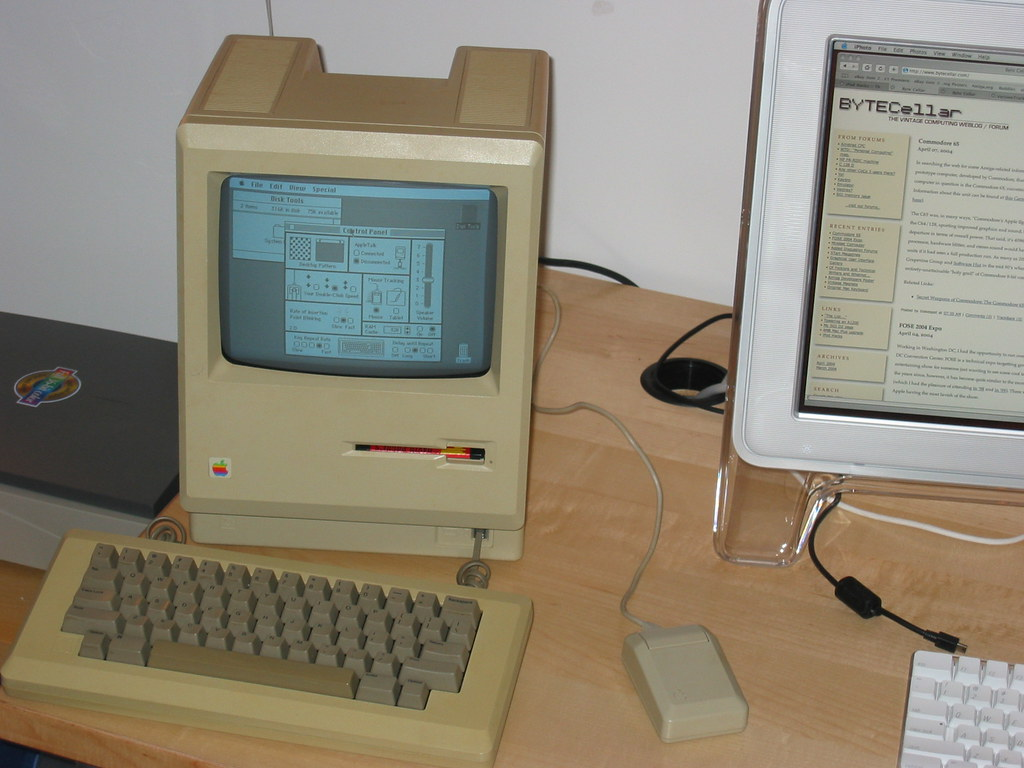
\includegraphics[width=0.6\textwidth]{figures/2388811229_7e3a50354d_b_d.jpg}
        \caption{Blake Patterson https://flic.kr/p/4D6hmv CC-By}
        \label{fig:gui}
    \end{figure}
   
\end{frame}

\begin{frame}{Command Line Interface}

    The Command Line Interface (CLI): Empty screen with a {\tt \$}. `Knowledge-in-the-head'\cite{Norman2013-xk}. Type instructions and computer executes quickly.

`The teletype would send that line to
the computer, which might or might not respond with some lines of its own, which the
teletype would hammer out–producing, over time, a transcript of your exchange with
the machine...' \cite{Stephenson1999-fw}

    
     \begin{figure}[H]

     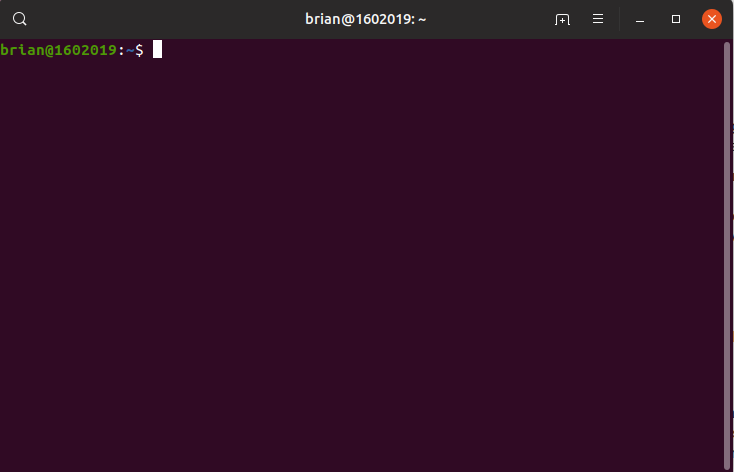
\includegraphics[width=.3\textwidth]{figures/terminal.png}
        \caption{Brian Ballsun-Stanton. CC0}
        \label{fig:cli}
        \end{figure}

\end{frame}

\begin{frame}{Nelle's Pipeline}

Nelle Nemo, a marine biologist, has just returned from a six-month survey of the North Pacific Gyre, where she has been sampling gelatinous marine life in the Great Pacific Garbage Patch. She has 1520 samples in all and now needs to:
\begin{enumerate}[label=\arabic*)]
    \item Run each sample through an assay machine that will measure the relative abundance of 300 different proteins. The machine’s output for a single sample is a file with one line for each protein.
    \item Calculate statistics for each of the proteins separately using a program her supervisor wrote called goostats.
    \item Write up results. Her supervisor would really like her to do this by the end of the month so that her paper can appear in an upcoming special issue of Aquatic Goo Letters.
\end{enumerate}

Two weeks to run 1520 samples.     

Using GUI would take 1520 different file selections. Finishing analysis would take longer than the month available.


As a bonus, once she has put a processing pipeline together, she will be able to use it again whenever she collects more data.
\end{frame}
% \begin{frame}{Assignment overview 2}
% \begin{itemize}[label=\textbullet]

% \item Learning Journal (Covered last week. Any technical work you do in this class should go into its own section). No formatting rules, though we disrecommend using word because it breaks things. (Due 4 times throughout semester)
% \item Lighting Talks (PICO Presentations) (Presenting your Proof of Concept (Tech Demo)) in a 2 minute mixed presentation/poster format. See EGU Pico presentation. (During exam time)
% \item Original Software Publication (Presenting your proof of concept as a paper which could be published in the SoftwareX Journal) (Due Week 13)
% \end{itemize}

% % Shawn, what visible thing will we change in reaction?
% \end{frame}

% \section{Jargon Busting}
% \begin{frame}{To open with, some jargon busting}
% Via @sheri: https://cloudstor.aarnet.edu.au/plus/f/3774955770

% Some terms of note:

% \begin{itemize}[label=\textbullet]
%     \item Proof of Concept (POC): `Assignment for FOAR705. See "Scoping", "Elaboration", "Deployment" A mechanism for describing, then creating a technology (tool and/or technique) workflow to assist your research.' The major work you will be doing over this semester. 
%     \item Typesetting: `Typesetting is the careful arrangement of text in a typeface in order to achieve maximum legibility,' \cite{Newcomb2019-hm}. The fourth step in the composition process (Preceded by Outlining (figuring out exactly what you want to say, and in what order, down to sub-paragraph detail), Writing, and Editing).
% \end{itemize}


% \end{frame}

% \section{Data Carpentry}
% \begin{frame}{Discussion from last week}

% Discussion:

% \begin{itemize}
% \item Episode 1:
% \begin{itemize}
% \item What was wrong with the SAFI `messy' data?
% \item What metadata should be recorded for the `clean' data?
% \end{itemize}
% \item Episode 2:
% \begin{itemize}
% \item What dirty data sets did you find?
% \item What errors did you find counterintuitive?
% \end{itemize}
% \end{itemize}



% \end{frame}
% \begin{frame}{Dates as Data}

% \begin{figure}[H]
%         \centering
%         \includegraphics[width=\textwidth]{figures/excel_dates_1.jpg}
%         \caption{Actual value in cells: `41822', `41834', and `1'. Dates as data, Data Carpentry. CC-By}
%         \label{fig:bigdates}
%     \end{figure}

% Also beware: Regional Date formatting.


% \end{frame}
% \begin{frame}{Exercise}

% Download and open the dates.xlsx file. This file contains a subset of the data from the SAFI interviews, including the dates on which the interviews were conducted.

% Choose the tab of the spreadsheet that corresponds to the way you format dates in your location (either day first {\tt DD\_MM\_YEAR }, or month first {\tt MM\_DD\_YEAR} ).

% Extract the components of the date to new columns. For this we can use the built in Excel functions:

% {\tt =MONTH()} 

% {\tt =DAY()}

% {\tt =YEAR()}

% Apply each of these formulas to its entire column. Make sure the new column is formatted as a number and not as a date.

% \end{frame}

% \begin{frame}{Exercise}
% Using the same spreadsheet you used for the previous exercise, add another data point in the {\tt interview\_date} column by typing either {\tt 11/17} (if your location uses {\tt MM/DD} formatting) or {\tt 17/11} (if your location uses {\tt DD/MM} formatting). The {\tt Day}, {\tt Month}, and {\tt Year} columns should populate for this new data point. What year is shown in the {\tt Year} column?
% \end{frame}

% \begin{frame}{Notes on Quality Assurance}

% \begin{itemize}[label=\textbullet]
%     \item Do one thing at a time.
%     \item Constrain inputs as much as you can.
%     \item Calculations should have validation/sanity checks.
% \end{itemize}
% \end{frame}

% \section{Computational Thinking}

% \begin{frame}{What is Computational Thinking?}

% Computers are good at some things. Mostly boring and repetitive things. 

% People are good at other things. Mostly creative and interesting things.

% Computers are fast but stupid. They need clear, step-by-step instructions (which they can then execute quickly).

% Computational thinking is an approach that lets you decide \textbf{what} computers are good for, and \textbf{how} to tell the computer to do what you want.

% \end{frame}

% \begin{frame}{Decomposition and algorithm design}

% \textbf{Computational Thinking }(CT) is a problem solving process that includes a number of characteristics and dispositions. \cite{Google2019-es}
% \begin{itemize}[label=\textbullet]
%     \item \textbf{Decomposition}: Breaking down data, processes, or problems into smaller, manageable parts.
%     \item \textbf{Algorithm Design}: Developing the step by step instructions for solving this and similar problems.
% \end{itemize}

% Bonus points for:
% \begin{itemize}
%     \item \textbf{Pattern Recognition}: Observing patterns, trends, and regularities in data.
%     \item \textbf{Abstraction}: Identifying the general principles that generate these patterns.
% \end{itemize}
% \end{frame}

% \begin{frame}{Computational Thinking example}

% 'I need to produce properly formatted references and bibliography in my thesis'

% [Articulate process in groups]

% \end{frame}

%  \section{Project management 101}

%  \begin{frame}{Developing ideas towards a solution}
%      So you have great ideas, what next? 
%  \end{frame}

%  \begin{frame}{Approach \#1: Top-down design (`Waterfall')}
%   \begin{figure}[Waterfall]
%      \centering
%          \includegraphics[height=.75\textheight]{figures/waterfall.png}
%          \caption{Traditional and linear approach \cite{Parody2018-if}} 
%          \label{fig:6}
%   \end{figure}
%  \end{frame}

%  \begin{frame}{Approach \#2: Iterative design with course corrections (`Agile')}
%   \begin{figure}[Agile]
%      \centering
%          \includegraphics[height=.75\textheight]{figures/agile.png}
%          \caption{Design-test-repeat approach to PM \cite{Parody2018-if}} 
%          \label{fig:7}
%   \end{figure}
%  \end{frame}

%  \begin{frame}{Manifesto for Agile Software Development}
%  We are uncovering better ways of developing software by doing it and helping others do it. Through this work we have come to value:
%      \begin{itemize}[label=\textbullet]
%          \item \textbf{Individuals and interactions} over processes and tools
%          \item \textbf{Working software} over comprehensive documentation
%          \item \textbf{Customer collaboration} over contract negotiation
%          \item \textbf{Responding to change} over following a plan
%      \end{itemize}
%  That is, while there is value in the items on the right, we value the items on the left more. \cite{Atlassian2019-xl}
%  \end{frame}

%  \begin{frame}{Tool \#1: Gantt chart}
%   \begin{figure}[Gantt]
%      \centering
%          \includegraphics[height=.75\textheight]{figures/gantt.png}
%          \caption{A Gantt Chart template (on Cloudstor)}
%          \label{fig:8}
%   \end{figure}
%  \end{frame}

%  \begin{frame}{Tool \#2: Kanban board}
%   \begin{figure}[Kanban]
%      \centering
%          \includegraphics[height=.75\textheight]{figures/kanban.png}
%          \caption{Schematic Kanban board \cite{Atlassian2019-bo}}
%          \label{fig:9}
%   \end{figure}
%  \end{frame}

%  \begin{frame}{A Kanban board should}
%      \begin{itemize}[label=\textbullet]
%          \item Visualise your work
%          \item Limit work in progress
%      \end{itemize}
%  Kanban boards often have columns like: Backlog (wish list), To do, In progress, Done, with the 'To do' and 'In progress' columns having work limits (e.g., 3-5 tasks). 

%  Trello is a popular application for Kanban. Atlassian has Kanban learning materials online \cite{Atlassian2019-bo}.
%  \end{frame}


\section{Minute cards!}
\begin{frame}{Feedback time}

On your green sticky, write one thing we did well today.

On your red sticky, write one thing we could improve upon for next time. Be specific. 

\end{frame}

\section{References}

\begin{multicols}{2}[]
\bibliography{references}
\bibliographystyle{apalike}
\end{multicols}


% \begin{frame}[allowframebreaks]{References}
  
%   \bibliography{references}
%   \bibliographystyle{apalike}
% \end{frame}


\begin{frame}{Thank you!}

% This presentation is available at:
% \texttt{https://osf.io/...}

Source code for this presentation is available at: \url{https://github.com/MQ-FOAR705/MQ-FOAR705-Week3}

This work is licensed under a Creative Commons Attribution 4.0 International License.

\end{frame}



\end{document}